
\documentclass{article}
\usepackage{graphicx}
\usepackage[top=3cm]{geometry}
\usepackage{tabularray}
\usepackage{afterpage}
\usepackage{amsmath}
\usepackage{listings}
\usepackage{subcaption}
\usepackage{mwe}
\lstset{language=Matlab}
\graphicspath{{./}}
\author{ Harshal Varpe}
\title{ECE 8540 Analysis of Tracking System\\
\Large Lab 5 Report: Extended Kalman Filter }

\begin{document}
\maketitle

\section{Introduction}\label{sec:intro}

In his lab report, we deal with implementing the Extended Kalman filter. A Kalman filter is an optimal filter used to optimally estimate the variables of interest that cannot be measured directly.
However Kalman filter works optimally when the system is linear, and the noise models are Gaussian. Although the Kalman filter can handle small non-linearities in the system, Extended Kalman Filter does a better job at handling non-linear systems. It is worth mentioning that both the Kalman Filter (KF) and the Extended Kalman Filter(EKF) work best when the noise models are Gaussian. Additionally, both KF  and EKF have some tolerance to non-Gaussian noise models.\\
For this lab, the students were provided with data of a sinusoid nature. The data file contained ground truth and the measurement. In the subsequent sections, we discuss the general mathematical model behind the EKF with the sinusoidal model and pseudo-code for the same. In the last section, we discuss the effects of dynamic noise and measurement noise on the performance of the EKF.\\

\section{Methods and Implementation}\label{sec:meth}
\subsection{EKF for Sinusoidal Model}
The Kalman filter functions in a continuous loop of predictions and updates. The whole cycle is explained below in terms of equations that can be implemented. For this example, the state variables are as follows:

\begin{equation}
\label{eqn:one}
X_t = \begin{bmatrix}
x_t \\
\dot{x}_t \\
h_t
\end{bmatrix}
\end{equation}

\indent
In equation \ref{eqn:one}, variable \textit{x} is similar to time and $\dot{x}$ is with dynamic noise $a_t$ represents uncertainty in the sinusoid over time. The variable \textit{h} provides the actual value of the sinusoid. \\
We can also write the state transition equations as follows:

\begin{equation}
\label{eqn:two}
f(x_t,a_t) = \begin{bmatrix}
x_{t+1} = x_t + \dot{x}_t T \\
\dot{x}_{t+1} = \dot{x}_t + a_t \\
h_{t+1} = \sin \frac{x_t}{10}
\end{bmatrix}
\end{equation}

\indent
In the state transition equations \ref{eqn:two} given above, $a_t$ is a random sample drawn from $N(0,\sigma_a^2)$ representing uncertainty in the propagation of the sinusoid over time. \\
\indent
For observation, we will assume a sensor that detects the current height of the sinusoid , $d_t$.
\begin{equation}
Y_t = \begin{bmatrix}
d_t
\end{bmatrix}
\end{equation}
\indent
The observation equations for this model are:
\begin{equation}
g(x_t,n_t) = \begin{bmatrix}
d_t = h_t + n_t
\end{bmatrix}
\end{equation}
\indent
where $n_t$ is a random sample drawn from $N(0,\sigma_n^2)$ representing measurement noise. \\

Now that we have defined the state transition equations, observation equations, and required variables, we now define the four Jacobians.
\\ \indent
The derivative of the state transition equations with respect to the state variables is: 
\begin{equation}
\label{eq: dfdx}
\frac{\partial f}{\partial x} =
\frac{\partial f}{\partial (x,\dot{x},h)} =
\begin{bmatrix}
1 & T & 0  \\
0 & 1 & 0  \\
\frac{1}{10} \cos \frac{x}{10} & 0 & 0 
\end{bmatrix}
\end{equation} \\
\\ \indent
The derivative of the observation equations with respect to the dynamic noises is:
\begin{equation}
\label{eq: dfda}
\frac{\partial f}{\partial a} =
\frac{\partial f}{\partial (0,a_t,0)} =
\begin{bmatrix}
0 & 0 & 0  \\
0 & 1 & 0  \\
0 & 0 & 0 
\end{bmatrix} 
\end{equation}
\indent
The derivative of the observation equations with respect to the state variables is:
\begin{equation}
\label{eq: dgdx}
\frac{\partial g}{\partial x} =
\frac{\partial g}{\partial (x,\dot{x},h)} =
\begin{bmatrix}
0 & 0 & 1
\end{bmatrix}
\end{equation}
The value of this Jacobian is calculated in each iteration. 
\indent
The derivative of the observation equations with respect to the measurement noises is:
\begin{equation}
\label{eq: dgdn}
\frac{\partial g}{\partial n} =
\frac{\partial g}{\partial (n_t)} =
\begin{bmatrix}
1 
\end{bmatrix}
\end{equation}
\\ \indent
The covariance of the dynamic noise is
\begin{equation}
Q = \begin{bmatrix}
0 & 0 & 0  \\
0 & \sigma_a^2 & 0  \\
0 & 0 & 0 
\end{bmatrix}
\label{eq: Q}
\end{equation}
\\ \indent
The covariance of the measurement noises is
\begin{equation}
R = \begin{bmatrix}
\sigma_n^2
\end{bmatrix}
\label{eq: R}
\end{equation}

In the end, we define the state estimate covariance $S_t$. This matrix represents the level of uncertainty in the state variables in \ref{eqn:one}. For our problem, the state estimate covariance is $S_t$:
\begin{equation}
S_t = \begin{bmatrix}
1 & 0 & 0 \\
0 & 1 & 0 \\
0 & 0 & 1 \\
\end{bmatrix}
\end{equation}

\subsection{MATLAB Implementation}

As previously mentioned the EKF is a continuous predict and update loop. The implementation of the filter for this problem is given below.  \\

\begin{enumerate}
\item Predict next state: 
\begin{equation}
X_{t,t-1} = f(X_{t-1,t-1},0)
\label{eq:}
\end{equation}
where $f(X_{t-1,t-1},0)$ is the approximated state $\tilde{x}_t$. \\
\item Predict next state covariance: 
\begin{equation}
S_{t,t-1} =
\left( \frac{\partial f}{\partial x} \right)
S_{t-1,t-1} \left(\frac{\partial f}{\partial x}\right)^T
+ \left( \frac{\partial f}{\partial a} \right) Q
\left(\frac{\partial f}{\partial a}\right)^T
\end{equation}
where $\left(\frac{\partial f}{\partial x}\right)$ and $\left(\frac{\partial f}{\partial a}\right)$ are the Jacobians of the state transition equations. \\
\\
\item Obtain measurement(s) $Y_t$ \\
\item Calculate the Kalman gain (weights)
\begin{equation}
K_t = S_{t,t-1} 
\left( \frac{\partial g}{\partial x} \right)^T
\left[
\left( \frac{\partial g}{\partial x} \right)
S_{t,t-1}
\left( \frac{\partial g}{\partial x} \right)^T
+
\left( \frac{\partial g}{\partial n} \right)
R
\left( \frac{\partial g}{\partial n} \right)^T
\right]^{-1}
\end{equation}
where $\left(\frac{\partial g}{\partial x}\right)$ and $\left(\frac{\partial g}{\partial n}\right)$ are the Jacobians of the measurement equations.

\item Update state
\begin{equation}
X_{t,t} = X_{t,t-1} + K_t [Y_t - g(\tilde{x}_t,0)]
\end{equation}
where $g(\tilde{x}_t,0)$ is the ideal (noiseless) measurement of the approximated state from above.

\item update state covariance
\begin{equation}
S_{t,t} = \left[ I - K_t
\left( \frac{\partial g}{\partial x} \right) \right] S_{t,t-1}
\end{equation}

\item Now increment the loop iterator \textit{t}
\end{enumerate}

It is important to note that the state covariance, dynamic noise covariance, and measurement noise covariance need to be defined at time 0. Moreover, it must be noted that the jacobian $\left(\frac{\partial f}{\partial x}\right)$ is not constant and must be calculated each iteration.

For this problem, the three different ratios of dynamic noise to measurement noise were tried. The following table shows the values of dynamic noise and measurement noise for each of the ratios.
\begin{center}
\begin{tabular}{| c | c | c |} 
 \hline
  & Q & R \\ [0.5ex] 
 \hline\hline
 Ratio 1 & 0.001 & 1  \\ [0.5ex]
 Ratio 2 & $10^{-10}$ & $ 10^{10}$ \\[0.5ex]
 Ratio 3 & 100 & 10 \\[0.5ex]
 \hline
\end{tabular}
\end{center}

\section{Result}\label{sec:code}

\indent

In figures \ref{fig:first} and \ref{fig:second}, we can see that the filtered estimate is much closer to the ground truth, and moreover, the estimate follows a general trend shown by measurement data. In this case, the values of dynamic and measurement noise are well balanced. Thus, we get an estimate that closely follows the ground truth.\\
\indent
In figures \ref{fig:third} and \ref{fig:fourth}, we see a plot of filtered estimate against the ground truth and measurement. Here the values of dynamic noise and measurement noise are  $10^{-10}$ and $10^{10}$, respectively. Since there is a huge difference between the dynamic and measurement noise, the estimate should closely reflect the small values of sin as shown in equation \ref{eqn:two}. Depending on how huge the difference is between dynamic and measurement noise, we will see a straight line with some or no oscillations. In our case, we see no oscillations.\\
\indent
From figures \ref{fig:fifth} and \ref{fig:sixth}, we see that the filtered estimate does a poor job of following the ground truth. However, the estimate tries to follow the measurement data.

In general, lower values of Q or dynamic noise mean that the Filter should trust more in state transition equations and not in the measurement data. Similarly, lower values for the measurement noise mean that the filter should trust the measurement data more. For example, for ratio 3 (Q = 100 and R = 10 ), we trust the measurement data more than the state transition equations. Hence, we obtain a plot or filter where the estimate is much closer to the measurement data.\\
\vspace{2cm}
\begin{figure}[!ht]
\centering
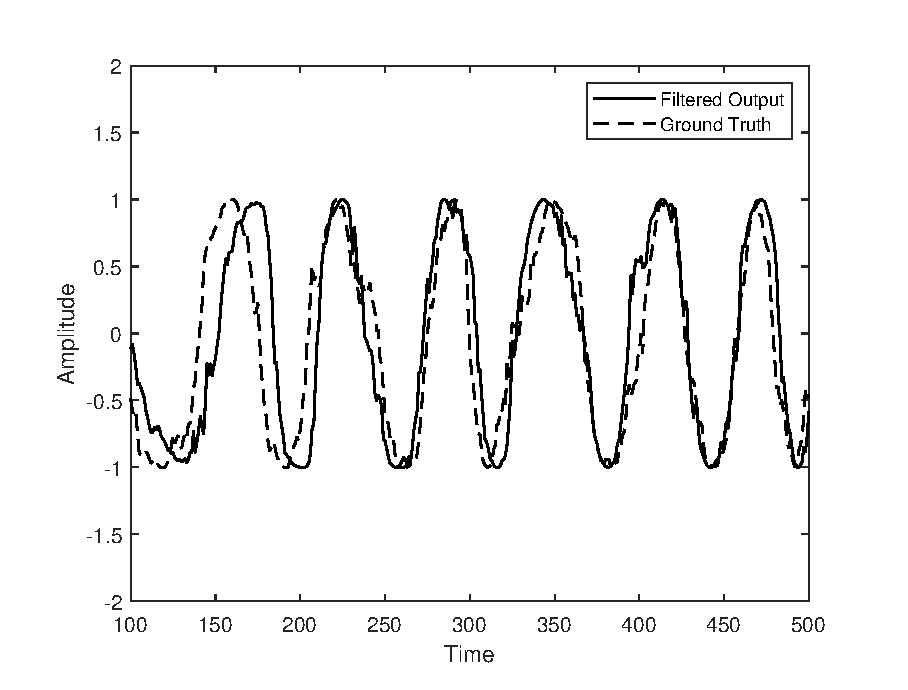
\includegraphics[scale=0.60]{ratio1_filt_vs_ground.eps}
\caption{Plot of Filtered estimate vs ground truth for ratio 1 (Q = 0.001 and R = 1)}
\label{fig:first}
\end{figure}

\begin{figure}
\centering
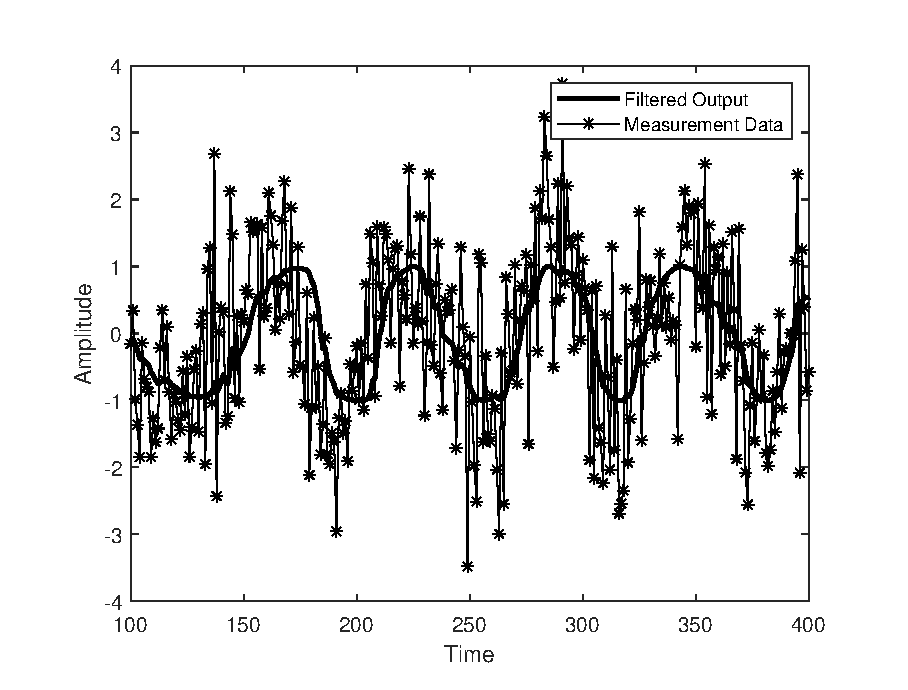
\includegraphics[scale=0.50]{ratio1_filt_vs_measure.eps}
\caption{Plot of Filtered estimate vs measurement for ratio 1 (Q = 0.001 and R = 1)}
\label{fig:second}
\end{figure}

\begin{figure}
\centering
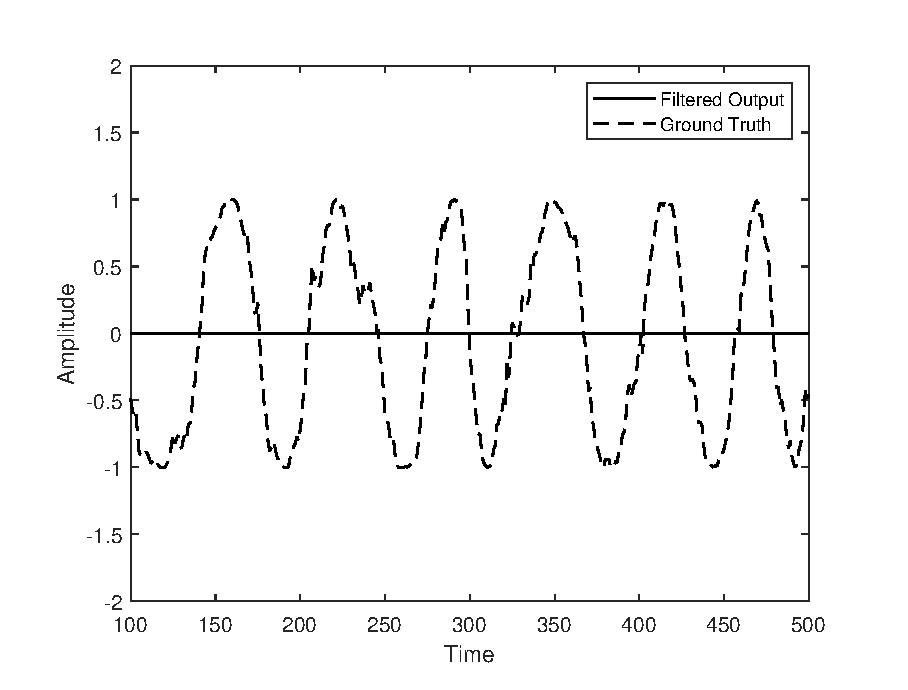
\includegraphics[scale=0.50]{ratio2_filt_vs_ground.eps}
\caption{Plot of Filtered estimate vs ground truth for ratio 2 (Q = $10^{-10}$ and R = $10^{10}$ )}
\label{fig:third}
\end{figure}

\begin{figure}
\centering
\includegraphics[scale=0.50]{ratio2_filt_vs_measure.eps}
\caption{Plot of Filtered estimate vs measurement for ratio 2 (Q = $10^{-10}$ and R = $10^{10}$ )}
\label{fig:fourth}
\end{figure}
\begin{figure}
\centering
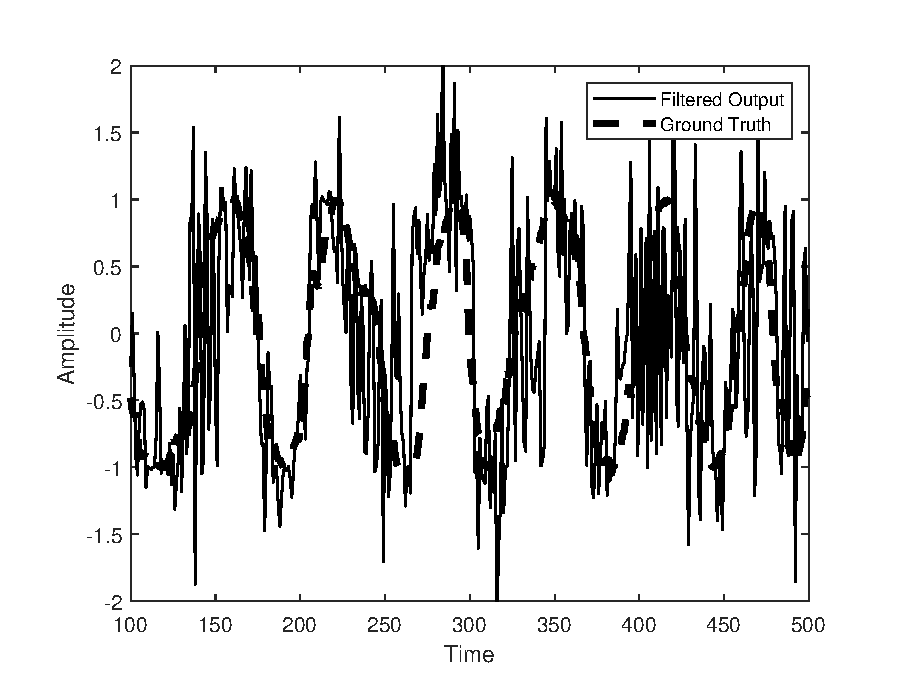
\includegraphics[scale=0.60]{ratio3_filt_vs_ground.eps}
\caption{Plot of Filtered estimate vs ground truth for ratio 3 (Q = 100 and R = 10)}
\label{fig:fifth}
\end{figure}
\begin{figure}
\centering
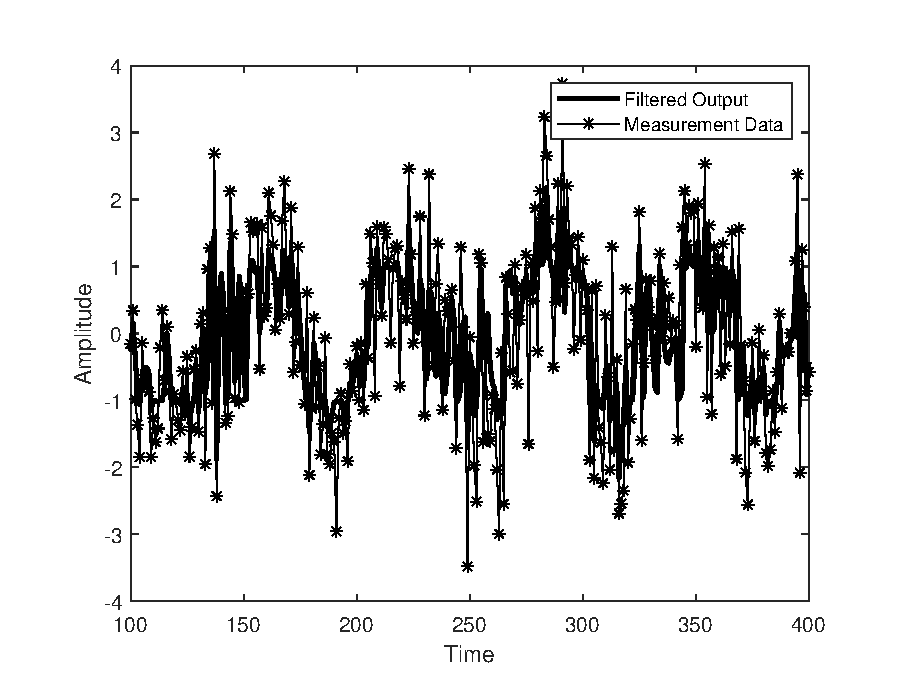
\includegraphics[scale=0.60]{ratio3_filt_vs_measure.eps}
\caption{Plot of Filtered estimate vs measurement for ratio 3 (Q = 100 and R = 10 )}
\label{fig:sixth}
\end{figure}



\pagebreak
\clearpage
\section{Conclusion}\label{sec:conc}

In summary, we can see that we have successfully implemented the Extended Kalman Filter. The extended Kalman filter tries to linearize any non-linearities in the model with the help of Jacobians. We also observed how the performance of the EKF changes as the ratio of dynamic noise to the measurement noise changes. Choosing optimal values for the dynamic noise and measurement noise falls on the designer of the filter. Fortunately, for the purpose of this lab, we had ground truth available, which helped determine the optimum values for the said quantities.

\section{Apendix}\label{sec:apdx}
 MATLAB code

\begin{lstlisting}[frame=single]

clc;
clear all;

data = importdata("data.txt");
ground_t = data(:,1);
measurements = data(:,2);

q = 0.001;
r = 1;

% q = 10^-10;
% r = 10^10;

% q = 100;
% r = 10;

dfda = [0 0 0; 0 1 0; 0 0 0];
dgdn = 1;
dgdx = [0 0 1];

Q = [0 0 0; 0 q 0; 0 0 0];
R = [r];

I = eye(3);
S = eye(3);
X = [0; 0; measurements(1)];

for t = 1:1:length(measurements)
    
    X_pred = [X(1)+X(2) ; X(2) ; sin(X(1)*0.1)];
    
%     X_pred = X ;
    
    dfdx = [1 1 0 ; 0 1 0 ; 0.1*(cos(X(1)*0.1)) 0 0];
    
    S_pred = dfdx * S * dfdx' + dfda * Q * dfda';
    
    Y = measurements(t);
    
    K = (S_pred * dgdx') / ((dgdx * S_pred * dgdx') + (dgdn * R * dgdn'));
    
    X = X_pred + K*(Y - X_pred(3));
    
    S = [I-K*dgdx]*S_pred;
    
    estimates(t) = X(3);
end
t = 1:1:length(measurements);


plot(t,estimates,"-k","linewidth",2)
hold on
% plot(t,ground_t,"--k","linewidth",3)
% hold on
plot(t,measurements,"-*k")
xlabel("Time");
ylabel("Amplitude");
% legend("Filtered Output","Ground Truth","Measurement Data");
% legend("Filtered Output","Ground Truth");
legend("Filtered Output","Measurement Data");
% legend("Ground Truth","Measurement Data");
% axis([0 780 -1.5 1.5])
% axis([0 780 -1.5 2])
axis([100 400 -4 4])
% axis([100 500 -2 2])

\end{lstlisting}


\end{document}